\section{Antecedentes y justificación}
Esta sección se centra en describir el ecosistema actual del desarrollo e investigación 
de modelos de inteligencia artificial y justificar la necesidad de la creación de un
estándar dentro de un equipo. Se presentan datos e información general sobre las 
tecnologías más relevantes utilizadas en el proyecto, dando una visión general 
de por qué se eligieron, teniendo en cuenta las últimas tendencias que están
surgiendo en el ámbito del aprendizaje automático.

\subsection{Justificación}
Cada año, más empresas y organizaciones invierten recursos significativos en 
proyectos de IA. Como se muestra en la figura \ref{fig:ai-investement},
en 2021 la inversión global superó los 270 mill millones de dólares \cite{Letzing2024-nn},
lo que supone un aumento del 40\% de la inversión con respecto al año anterior.
Este crecimiento de la inversión busca aprovechar al máximo el potencial de la IA 
y sacar provecho de su ventaja competitiva. Un ejemplo notable de este fenómeno es OpenAI, 
una empresa que ha sido valorada en más de 80 mil millones de dólares \cite{noauthor_2024-uj} con el record de crecimiento 
en el numero de usuarios más rápido de la historia \cite{Armenta2023-xt}. Todo esto
gracias a su modelo de lenguaje GPT-3 y sus respectivas versiones GPT-4, GPT4-turbo y GPT4-o, 
que han demostrado cómo una aplicación de inteligencia artificial puede llegar a
impactar significativamente en la vida de las personas.

\begin{figure}[ht]
    \centering
    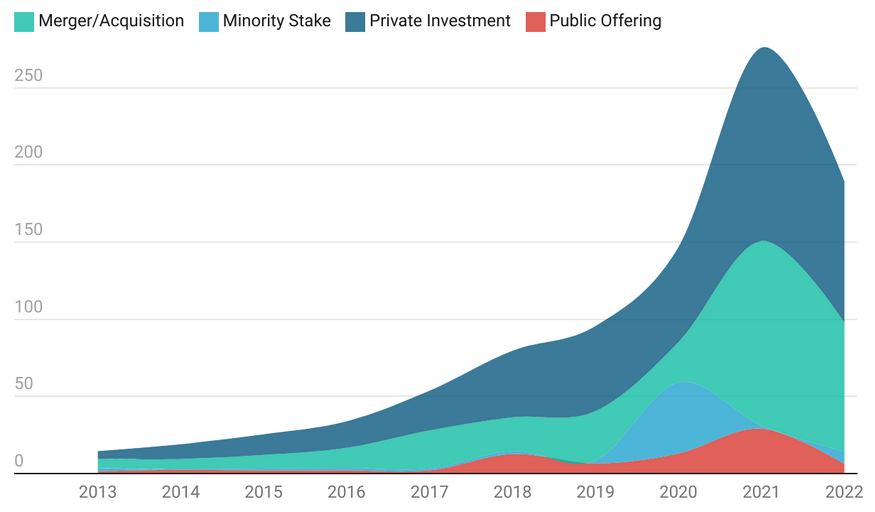
\includegraphics[width=\textwidth]{ai-investement.png}
    \caption{Inversión global en IA en miles de millones \cite{Letzing2024-nn}.}
    \label{fig:ai-investement}
\end{figure}

La demanda de equipos cualificados en el desarrollo de modelos de IA 
que puedan hacer frente a los nuevos desafíos es mayor que nunca. La complejidad
de los proyectos de IA está en aumento, ya que las aplicaciones de IA
se vuelven más sofisticadas, abarcan una gama más amplia de funciones, requieren
un mayor número de datos y los modelos se vuelven cada vez más complejos. Esta
situación ha forzado a las empresas a buscar nuevas formas de gestionar sus proyectos
que han llevado a la creación de nuevas metodologías, adaptadas a las necesidades
a los nuevos retos que se presentan. Si bien es cierto que mucha información es
compartida con la comunidad, existe un gran secretismo en torno a la forma de operar
de las empresas más grandes, lo que dificulta la adopción de estas metodologías.
Podemos resaltar positivamente el caso de Meta \cite{metaia}, que es el mayor 
referente en cuanto contribución y apertura de sus desarrollos en IA.\medskip

Por todo ello, es necesario realizar contribuciones que se centren en el como 
se debería operar dentro de un equipo. Se requiere de una referencia clara sobre las 
directrices que se deben aplicar para poder implementar un estándar tecnológico y
operacional dentro de un grupo de trabajo, así como las herramientas, metodologías y buenas prácticas
a seguir para hacer un uso eficiente de los recursos y obtener resultados de calidad.
Este documento representa un estándar que se ha aplicado en base a unas necesidades
concretas y, aunque no está pensado para poder ser adoptado de forma literal por otros equipos,
se muestra el camino que se ha seguido desde la adopción de plataformas MLOps hasta la creación
de un sistema de conocimiento para la reutilización de trabajo. La justificación de este
documento es exponer el trabajo realizado y servir como referencia equipos que quieran implementar
un estándar similar o busquen inspiración para crear el suyo propio.
 
%% Antecedentes -> Contenido general
%% Estado del arte -> Contribuciones de otros equipos
%% Referencias sobre replicabilidad 

\subsection{Antecedentes}
En la sección de antecedentes, se profundiza en aquellos conceptos esenciales que son 
indispensables para entender el alcance y las contribuciones de este trabajo, así como 
para situarlo dentro de un marco conceptual adecuado. Se abordan aspectos fundamentales 
que no solo proporcionan contexto, sino que también establecen las bases teóricas y 
metodológicas sobre las cuales se construye la investigación.

\subsubsection{Diseño Atómico}
El diseño atómico es una metodología de diseño que se centra en la creación
de sistemas modulares y reutilizables. La idea principal es dividir
las diferentes funcionalidades de un sistemas en sus partes más fundamentales,
de manera que cada una de estas partes pueda ser reutilizada en diferentes
contextos. Este enfoque permite tener un mayor control sobre cada una de las
partes del sistema, facilitando su mantenimiento, documentación y reutilización.
Originalmente, el diseño atómico ha sido aplicado en el diseño de interfaces
de usuario, pero su filosofía puede ser aplicada a cualquier sistema de diseño
modular. En el contexto de este proyecto, el diseño atómico se aplicará al
diseño de un sistema de componentes para el desarrollo de modelos de aprendizaje
automático.\medskip

Dentro del diseño atómico, los componentes se dividen en cinco categorías
principales, que representan diferentes niveles de abstracción. Estas categorías
son: átomos, moléculas, or\-ga\-nis\-mos, plantillas y páginas. Cada una de estas
categorías representa un nivel de abstracción diferente, y se relaciona con
las demás categorías de manera jerárquica. La figura \ref{fig:atomic-design}
muestra la estructura conceptual del diseño atómico.\medskip

\begin{figure}[ht]
    \centering
    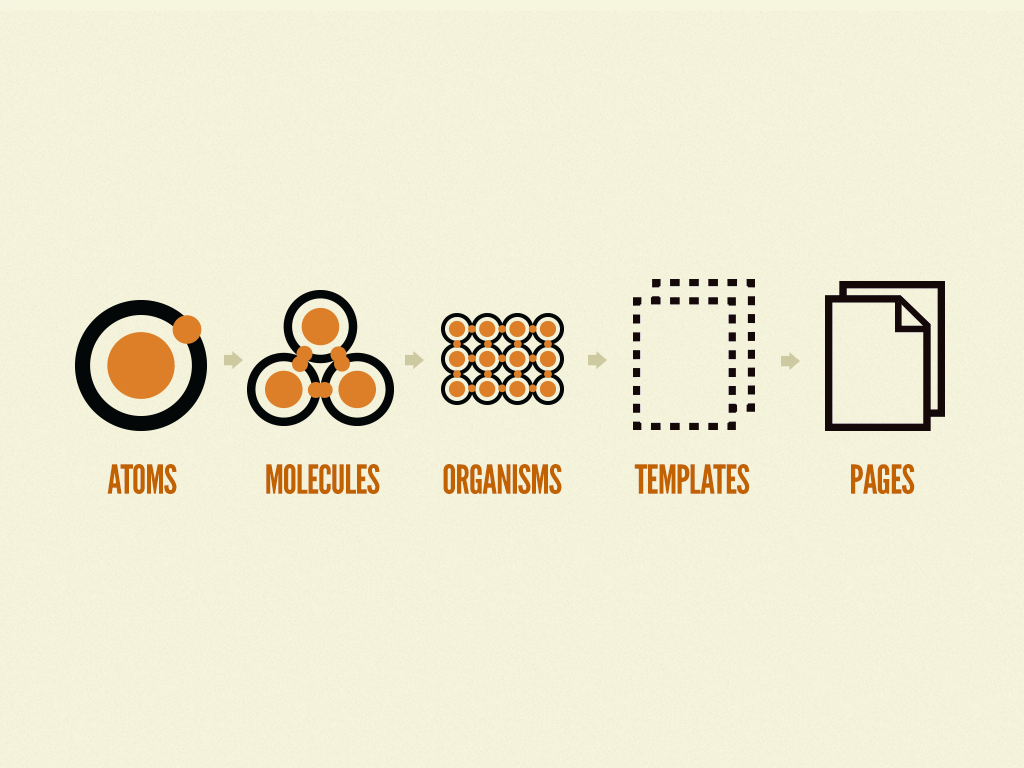
\includegraphics[width=0.7\textwidth]{atomic-design-process.png}
    \caption{Estructura conceptual diseño atómico \cite{frost2016atomic}.}\label{fig:atomic-design}
\end{figure}

A continuación, se describen brevemente cada una de las categorías:
\begin{itemize}
    \item \textbf{Átomos:} Los átomos son los componentes más básicos de un sistema
    de diseño. Representan las funcionalidades más fundamentales, solo tienen
    una responsabilidad y no dependen de otros componentes.
    \item \textbf{Moléculas:} Las moléculas son la combinación de varios átomos
    para formar una funcionalidad más compleja. Representan la combinación de
    diferentes funcionalidades básicas para formar una funcionalidad más compleja.
    \item \textbf{Organismos:} Los organismos son la combinación de varias moléculas
    y átomos para formar una funcionalidad completa.
    \item \textbf{Plantillas:} Las plantillas son la combinación de varios Organismos
    para dar forma a un contenido.
    \item \textbf{Páginas:} Las páginas son la combinación de varias plantillas.
\end{itemize}

Esta estructura jerárquica permite que los componentes sean reutilizados en
diferentes contextos, y que cada uno de ellos pueda ser modificado de manera
independiente. Además, se facilita la documentación y el mantenimiento de los
componentes, ya que cada uno de ellos es independiente de los demás. Podemos
ver multitud de ejemplos de diseño atómico en grandes empresas y que nosotros utilizamos
a diario, como por ejemplo en la creación de sistemas de diseño Microsoft Fluent
Design o Google Material Design entre otros.\medskip

Aunque el diseño atómico se ha aplicado tradicionalmente a la creación de interfaces
de usuario, su filosofía puede ser aplicada a cualquier sistema de diseño modular.
En el contexto de este proyecto, el diseño atómico se aplicará para la creación de un
sistema de componentes en el desarrollo de modelos de aprendizaje automático.
Traeremos la filosofía del diseño atómico y la adaptaremos a nuestro contexto,
con las particularidades y necesidades que requiere el desarrollo de modelos de
aprendizaje automático. 

\subsubsection{Machine Learning Operations (MLOps)}
El desarrollo de modelos de aprendizaje automático es un proceso complejo que implica
la recopilación de datos, la creación de modelos, la evaluación de los modelos y su
puesta en producción. Cada una de estas etapas requiere de diferentes herramientas y
prácticas, y es importante que estas herramientas y prácticas estén integradas de manera
coherente para garantizar la eficacia del proceso. Los principios de MLOPs son una serie de prácticas y herramientas que se utilizan
para gestionar el ciclo de vida de los modelos de aprendizaje automático. Como se muestra en la
figura \ref{fig:mlops-workflow}, este enfoque busca aplicar las mejores tendencias dentro de la 
ingeniería de software al desarrollo de modelos, con el objetivo de mejorar la eficiencia, la 
calidad y la escalabilidad.\medskip

\begin{figure}[ht]
    \centering
    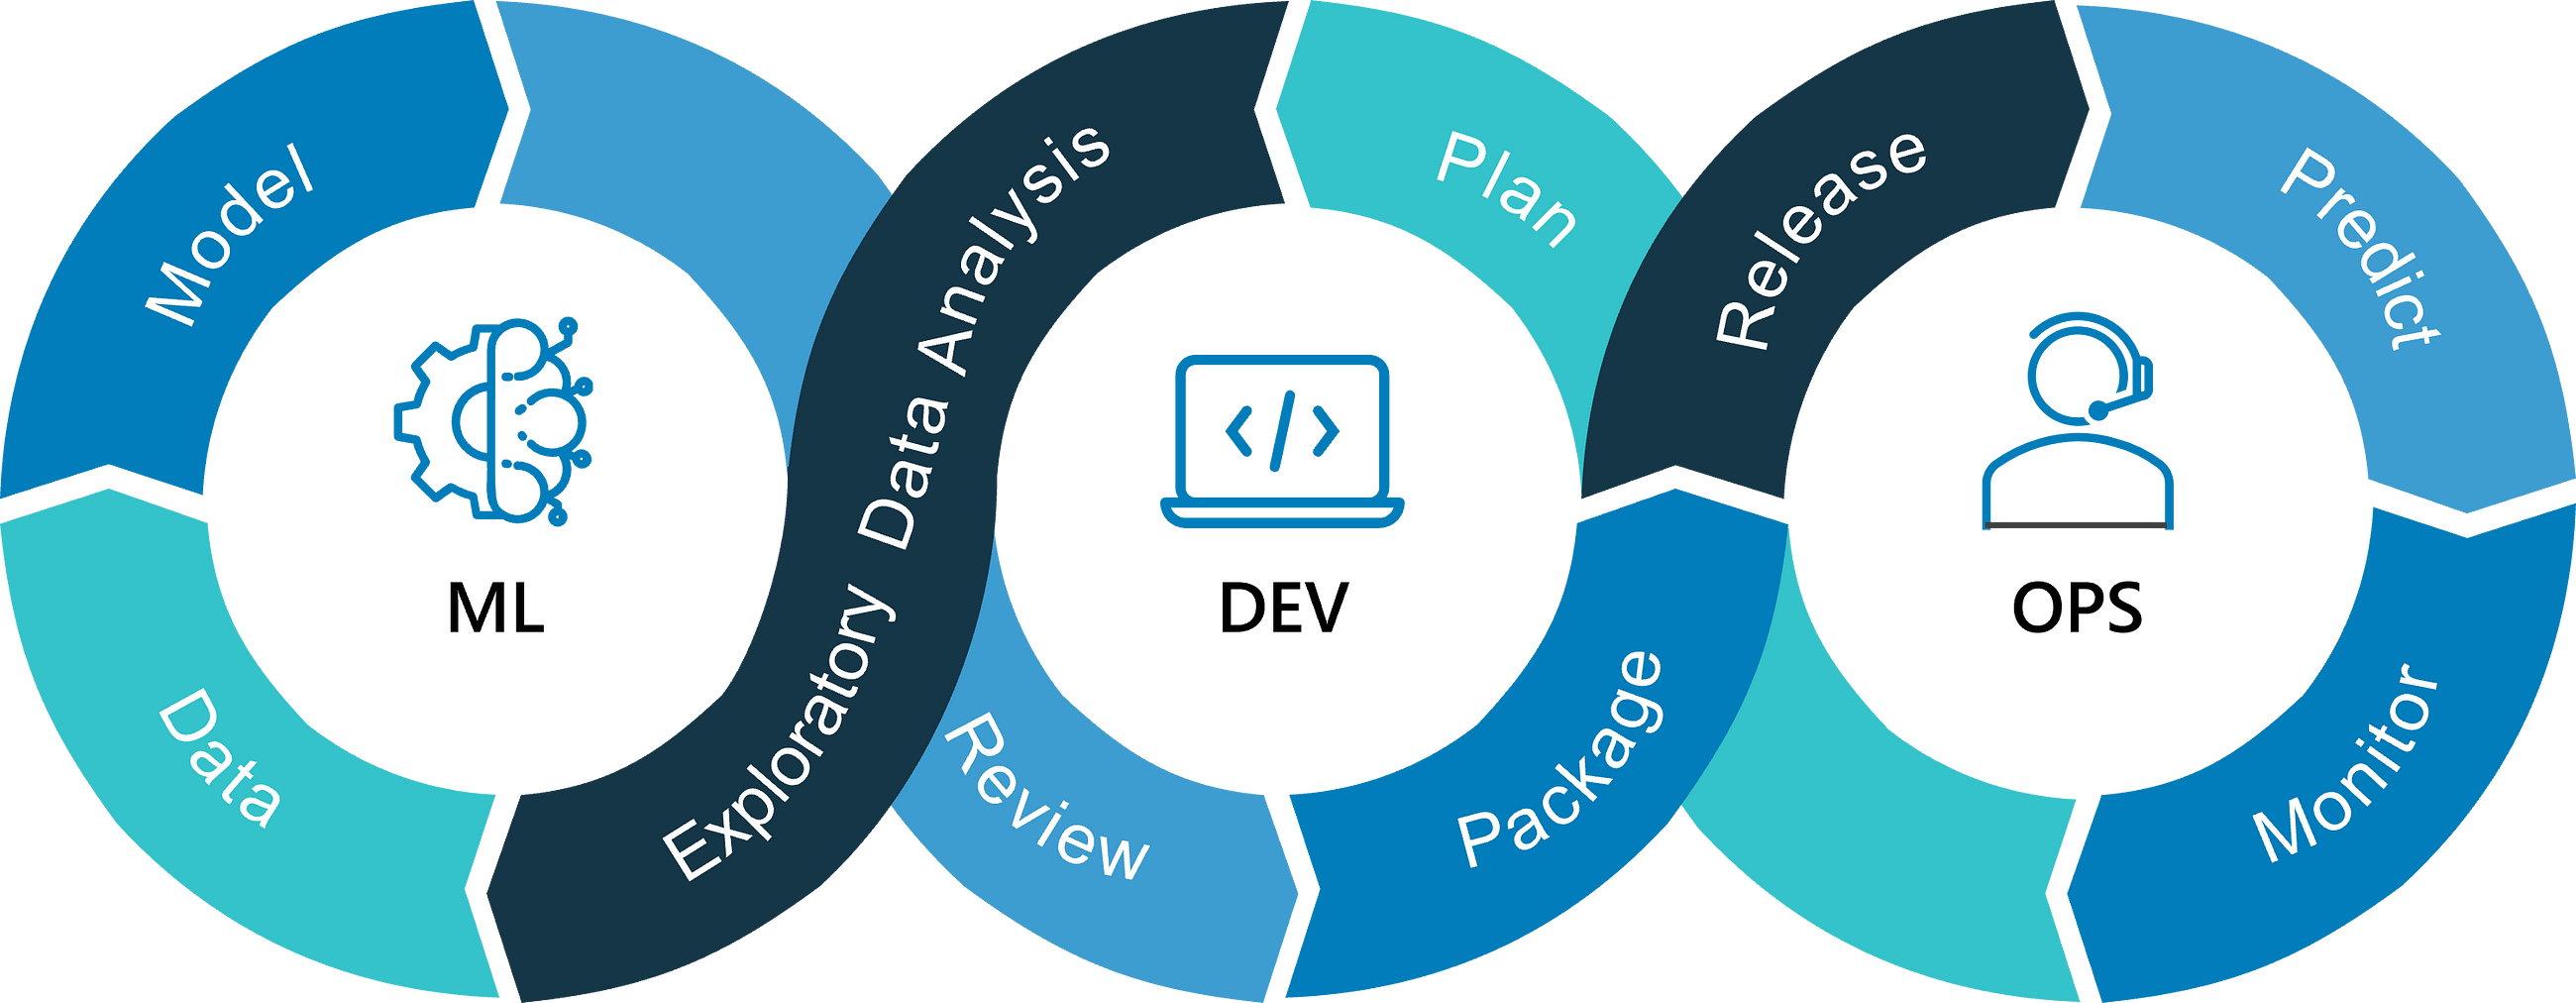
\includegraphics[width=\textwidth]{mlops-workflow.png}
    \caption{Ciclo de vida MLOps \cite{Merritt_2020}.}\label{fig:mlops-workflow}
\end{figure}


Algunos de los principios clave de MLOps son:

\begin{itemize}
    \item \textbf{Automatización:} la automatización es esencial para mejorar la eficiencia del
    desarrollo de modelos y prevenir errores. Esto implica automatizar tareas como la 
    generación de datos, el despliegue de modelos, evaluación y su puesta en producción.
    \item \textbf{Colaboración y reproducibilidad:} uno de los desafíos en el aprendizaje automático es lograr 
    reproducir resultados de manera consistente, dada la naturaleza aleatoria de los algoritmos.
    MLOps busca, en la medida de lo posible, garantizar cierta consistencia entre los resultados
    obtenidos durante diferentes ejecuciones de un modelo para facilitar la colaboración entre
    los miembros del equipo.
    \item \textbf{Monitorización:} una vez que un modelo está en producción, es importante monitorizar
    su rendimiento para garantizar su eficacia y detectar posibles problemas. La monitorización
    permite crear alertas en caso de que el modelo no funcione correctamente y tomar medidas
    para corregirlo como por ejemplo, actualizar el modelo con nuevos datos.
    \item \textbf{Gestión de versiones:} controlar las versiones de los modelos y los datos es esencial
    para garantizar la reproducibilidad y la trazabilidad de los modelos. La gestión de versiones
    permite a los equipos comprender cómo ha evolucionado un modelo a lo largo del tiempo e incluso
    retroceder a versiones anteriores fuera necesario.
\end{itemize}

\subsection{Estado del arte}
La sección de estado del arte se centra en estudiar y analizar las tendencias
actuales dentro del ámbito del aprendizaje automático y la inteligencia artificial.
Debido a la diversidad de ramas que abarca la creación de un estándar tecnológico y
operacional, se han seleccionado aquellas que se consideran más relevantes o presentan
un mayor peso en cuanto a la toma de decisiones.

\subsubsection{Irrupción de las metodologías ágiles}
La aparición de metodologías ágiles en el desarrollo de software, con sus numerosas ventajas, 
ha dejado en desuso muchas metodologías clásicas. Las metodologías ágiles introdujeron el 
concepto de DevOps como un cambio de mentalidad \cite{salvucci2021mlops} 
en la que los diferentes equipos colaboran para implementar procesos más rápidos y 
entregar nuevas funcionalidades al cliente de manera más ágil. MLOps es una extensión de 
DevOps que ha surgido muy recientemente y, por lo tanto, existen pocos estudios que 
aborden el tema \cite{kreuzberger2022mlops}\cite{recupito2022multivocal}.\medskip

Principalmente existen dos formas para implementar MLOps en una organización, uno es
a través de los sistemas cloud que ofrecen servicios MLOps como Azure ML \cite{microsoft2023azureml}, 
AWS Sagemaker \cite{aws_sagemaker} o Google Cloud Vertex AI \cite{google2023vertexai}. El otro es a través del despliegue de una plataforma open source
como MLFlow dentro de la infraestructura propia. Las principales diferencias entre ambas
opciones son el coste y la flexibilidad, ya que los servicios cloud ofrecen una mayor
facilidad de uso y mejor experiencia de desarrollo, pero a un coste mayor. Por otro lado,
la implementación de una plataforma open source requiere de un mayor esfuerzo pero ofrece
se recompensa con una mayor flexibilidad y control sobre la infraestructura.

\subsubsection{Problemas de replicabilidad}
La crisis de replicabilidad es un fenómeno crítico en la comunidad científica,  
donde los resultados de los estudios a menudo no pueden replicarse con nuevos datos \cite{puetz2024replication}.
Este problema es muy destacado en numerosos campos científicos, que se han enfatizado particularmente 
en disciplinas como la psicología, la salud y la medicina \cite{puetz2024replication}\cite{Baker_2016}, donde hallazgos incorrectos 
podrían tener consecuencias graves. Durante los últimos años, la crisis de replicabilidad ha
sido objeto de debate dentro de la rama de la inteligencia artificial, donde la falta de
transparencia, la complejidad de los modelos y la imposibilidad de replicar los resultados
han sido identificados como problemas clave.

\begin{figure}[ht]
    \centering
    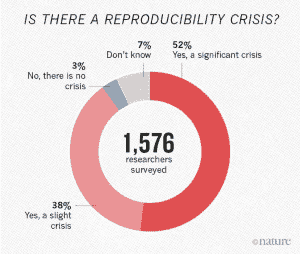
\includegraphics[width=0.75\textwidth]{crisis-survey.png}
    \caption{Recreación gráfico crisis de reproducibilidad en la ciencia \cite{Baker_2016}}\label{fig:crisis-survey}
\end{figure}

La confusión se ve incrementada por el uso variado de términos clave como reproducibilidad, 
replicabilidad y repetibilidad, \cite{readytensor} dificultando los esfuerzos para abordar estos problemas de 
manera efectiva. Se definen los diferentes términos de la siguiente manera:
\begin{itemize}
    \item \textbf{Repetibilidad:} se centra en la consistencia de los resultados de la investigación cuando el equipo 
    original re-ejecuta su experimento bajo condiciones inalteradas. 
    \item \textbf {Reproducibilidad:} se logra cuando investigadores independientes validan los hallazgos del 
    experimento original empleando el documentado original. Esta validación puede ser directa, utilizando 
    los datos y el código originales, o independiente, a través de la reimplementación del experimento, 
    probando así la fiabilidad de los resultados en diferentes equipos.
\end{itemize}

Una serie de estudios y encuestas subrayan la gravedad de la situación \cite{Baker_2016}.
Como se muestra en la figura \ref{fig:crisis-survey}, una encuesta realizada a 1500 investigadores
encontró que el 50\% de ellos afirman que que hay una crisis significativa y un 40\% que hay
una crisis moderada, dejando solo un 10\% que no ve una crisis en la replicabilidad de los estudios.
Existen multitud de casos donde los intentos de volver a ejecutar experimentos dan como resultado 
a una amplia desviación, incluso bajo condiciones idénticas\ref{fig:crisis-survey}.
Los propios investigadores tienen dificultades para reproducir sus propios experimentos.
La figura \ref{fig:self-reproduce} nos da una idea de lo frecuente que es este problema,
donde en el caso de la física e ingeniería, el 50\% de los encuestados han tenido problemas
reproduciendo sus experimentos, lo que se ve reflejado en que el 70\% de ellos haya tenido
problemas al intentar reproducir los experimentos de otros investigadores.

\begin{figure}[ht]
    \centering
    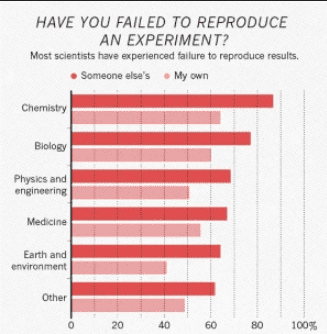
\includegraphics[width=\textwidth]{self-reproduce.png}
    \caption{Problemas con la reproducibilidad por disciplina \cite{Baker_2016}}\label{fig:self-reproduce}
\end{figure}

Estos problemas se consideran como los principales causantes como se puede ver en la figura \ref{fig:repro-factor}.
Factores como la falta de información sobre detalles experimentales y los tiempos de pu\-bli\-cación, enfatizando 
la necesidad urgente de un enfoque más sistemático y transparente. Sin contar los problemas
directamente relacionados con el desarrollo, como son la procedencia y calidad de los datos, la 
elección del algoritmo, el hardware utilizado para su entrenamiento, el preprocesamiento de 
los datos, entre otros.

\begin{figure}[ht]
    \centering
    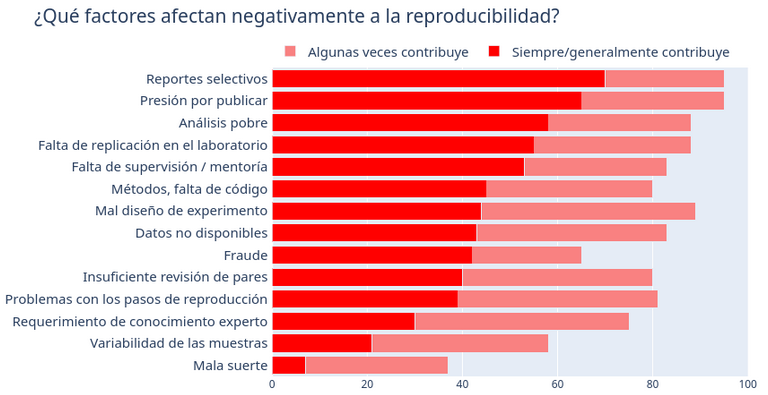
\includegraphics[width=\textwidth]{repro-factor.png}
    \caption{Factores que contribuyen a la irrepoducibilidad \cite{Baker_2016}}\label{fig:repro-factor}
\end{figure}

Aunque la reproducibilidad es un problema complejo y multifacético, existen
algunas medidas que pueden tomarse para abordarlo. Algunas de estas medidas que encontramos
en al literatura son una mejor supervisión, mejora del proceso de validación, incentivar
buenas practicas de desarrollo, entre otras. 

\subsubsection{Calidad del software y buenas prácticas}
Las buenas prácticas en la programación, como el uso de patrones de diseño, la 
creación de tests y una documentación adecuada, son esenciales para asegurar un 
alto rendimiento y eficiencia en los sistemas de software. Estas prácticas no solo facilitan 
la colaboración entre los desarrolladores, sino que también ayudan a prevenir errores y 
mejorar la calidad del software producido. Se han encontrado evidencias \cite{Athanasiou2014Test} 
que sugieren que la detección y resolución temprana de problemas mejora significativamente a mayor sea la
cantidad y calidad de las pruebas realizadas. Este tipo de prácticas son especialmente importantes
ya que aseguran que el software desempeñe correctamente la función para la que fue diseñado y
permite tener un control mas en profundidad del mismo.\medskip

Dentro del campo del aprendizaje automático, la calidad del software es un aspecto crítico 
que puede afectar significativamente el rendimiento de los modelos. Pese a que estos sistemas
son más complejos y difíciles de depurar, debido a que muchos los modelos son en su mayoría
complejos en cuanto a explicabilidad, una mala gestión del código puede llevar a errores
de diferente índole. Identificar y comprender estos fallos es crucial para mejorar la calidad y fiabilidad de 
los sistemas de IA.\medskip

Los principales fallos relacionados con malas prácticas de código son los siguientes:

\begin{itemize}
    \item \textbf{Introducción de sesgos}: la proliferación de tecnologías 
    de minería de datos y la acumulación de datos sociales han llevado a su uso en 
    decisiones cruciales que afectan la vida de las personas\cite{kamishima2012fairness}. Este tipo de datos son
    muy complejos ya que la mayoría de veces carecen de consistencia, están entrelazados
    y ramificados, y son muy sensibles a los cambios. Es muy sencillo cometer errores en cuanto
    a la recolección y tratamiento de los datos, lo que puede llevar a la introducción de sesgos
    de manera inconsciente \cite{galhotra2017fairness}. Además, es necesario de conocimientos
    avanzados de tratamiento ya que muchas veces la práctica común de eliminar ciertos datos
    puede no ser suficiente para reducir el sesgo \cite{kamishima2012fairness}.
    \item \textbf{Uso excesivo de recursos:} El uso ineficiente 
    de recursos computacionales durante el entrenamiento y despliegue de modelos puede llevar a un gasto 
    innecesario de tiempo y energía \cite{Jun2010Comparative}. La optimización de algoritmos y la implementación de 
    técnicas de programación eficiente son esenciales para minimizar estos costos. Algunas de
    las prácticas que más impacto tienen en la eficiencia de los modelos son el uso de librearías
    basadas en C \cite{1182968}, la compilación de modelos mediante JIT \cite{Aycock2003Brief}, el empleo de técnicas de cacheo en
    momentos críticos \cite{lruCache}, entre otros. Estas practicas pueden suponer un aumento de la velocidad de
    ejecución de un x2 en el peor de los casos y un x4 de media \cite{Jun2010Comparative}. 
    \item \textbf{Errores en producción:} Los errores que no se detectan durante 
    la fase de desarrollo pueden manifestarse en entornos de producción, afectando la fiabilidad 
    y el rendimiento del sistema. La implementación de un sistema robusto de pruebas y monitoreo 
    continuo puede ayudar a identificar y solucionar estos problemas antes de que impacten a los 
    usuarios finales. Algunas de las practicas recomendables se basan el uso de librearías de validación como
    Pydantic \cite{pydantic}, que permiten validar los datos de entrada en tiempo real,
    la implementación de tests unitarios mediante Pytest \cite{Pytest} y la monitorización
    de los modelos en producción mediante herramientas como Prometheus \cite{prometheus} y Grafana \cite{grafana}.

\end{itemize}

% Vocales con acento -> áéíóú
 
\pagebreak